\section{ANEXOS}
\subsection*{ANEXO A: Explicación de los hiperparámetros y resultados de YOLO}
\label{subsec:A}

Las redes neuronales como \texttt{YOLO} y en general todas las que utilizan entrenamiento supervisado, tienen como objetivo acercarse lo máximo posible al resultado esperado en las etiquetas de entrenamiento. 
A lo largo de este entrenamiento se van actualizando parámetros (valores que sí cambian en entrenamiento) como son los pesos, los \texttt{bias} y otros elementos. Esta búsqueda de aproximación se puede ver 
reflejada como la búsqueda de mínimos globales en una función, en la mayoría de casos es buscar los mínimos globales de la función de perdidas. Esto se puede ver en la \autoref{fig:GradientDescendGlobales}.

\begin{figure}[H]
    \centering
    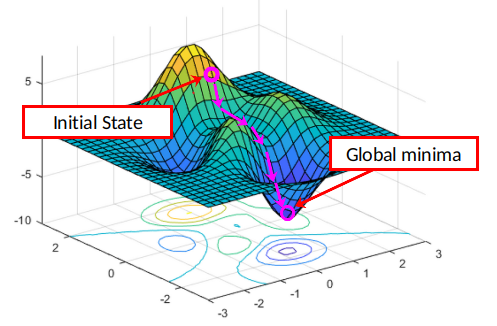
\includegraphics[width=0.5\textwidth]{images/13/a/GradientDescend.png}
    \caption{Búsqueda de mínimos globales por un algoritmo de aprendizaje automático\cite{doleronDeepLearningScratch2023}}
    \label{fig:GradientDescendGlobales}
\end{figure}

Los modelos de \texttt{YOLO} tienen definidos una serie de hiperparámetros (valores que no cambian en entrenamiento) que sirven como ajustes fijos durante en el entrenamiento. 
Estos hiperparámetros ajustan la manera en la que el algoritmo decide el siguiente paso a tomar en su búsqueda de un mínimo global y pueden acelerar o ralentizar el tiempo necesario 
de entrenamiento para alcanzar unos valores de perdida adecuados. Algunos de los hiperparámetros más típicos\cite{ultralyticsConfiguration} son:

\begin{itemize}
    \item \textbf{Learning Rate inicial}: es el valor que afecta cuanto se cambian los pesos entre época. Por defecto es \texttt{0.01}, que puede parecer poco, pero es mejor dar pasos pequeños para llegar al mínimo global.
    \item \textbf{Learning Rate final}: es una fracción del valor inicial. Cuanto más se entrena la red es normal reducir el \texttt{Learning Rate} para ajustar de forma más fina. Por defecto es \texttt{0.01}.
    \item \textbf{Momentum}: es una variable que permite tener en cuenta que camino se ha recorrido en la anterior época, para no volver a situaciones anteriores y seguir progresando. Por defecto es \texttt{0.937}.
    \item \textbf{Weight Decay}: hiperparámetro para prevenir sobreajuste y penalizar los pesos que son extremadamente grandes en la red.
    \item \textbf{Épocas de calentamiento}: número de épocas que se utilizaran para ir poco a poco acercándose a los valores iniciales de \texttt{Learning Rate}. Por defecto su valor es 3.
    \item \textbf{Tamaño de lote}: número de imágenes que se utilizaran en una pasada. Si tenemos 50 imágenes y el tamaño del lote es 10, se pasaran 10 y se ajustaran los pesos, y en este caso una época se compondra 
    de 5 pasadas de lote.
    \item \textbf{Número de épocas}
    \item \textbf{Número de capas ocultas}
\end{itemize}
\clearpage
Además, \texttt{YOLO} utiliza de base una herramienta de aumento de datos simple, por lo tanto tenemos muchos hiperparámetros para ajustar su funcionamiento:

\begin{itemize}
    \item \textbf{Hsv componente h}: ajusta el \texttt{Hue} de la imagen por una fracción que por defecto es \texttt{0.015}.
    \item \textbf{Hsv componente s}: ajusta la saturación de la imagen por una fracción que por defecto es \texttt{0.7}, permite simular diferentes condiciones de iluminación.
    \item \textbf{Hsv componente v}: modifica el brilo de la imagen, por defecto a una fracción de \texttt{0.4}.
    \item \textbf{Translate}: mueve la imagen horizontal y verticalmente por defecto un \texttt{10\%}.
    \item \textbf{Scale}: ajusta el tamaño de la imagen para simular diferentes distancias a la cámara. Por defecto \texttt{0.5}.
    \item \textbf{Fliplr}: espeja la imagen horizontalmente con una probabilidad por defecto de \texttt{0.5}.
    \item \textbf{Mosaic}: permite combinar 4 imágenes en una para crear imágenes compuestas que mejoran mucho la calidad del entrenamiento. Por defecto siempre está activo.
    \item \textbf{Erasing}: borra partes de la imagen de forma aleatoria para que el modelo sepa reconocer segmentos del elemento y que sea capaz de detectar características más específicas.
    \item \textbf{Crop fraction}: de forma aleatoria corta la imagen a fracciones de su tamaño original.
\end{itemize}
El resultado de este aumento de datos se puede ver en los lotes con los que se entrena la red como el de la \autoref{fig:AumentoDatosYolo}, donde vemos cambios de brillo, saturación, recortes de imagen y 
combinación de imágenes en diferentes tamaños.
\begin{figure}[H]
    \centering
    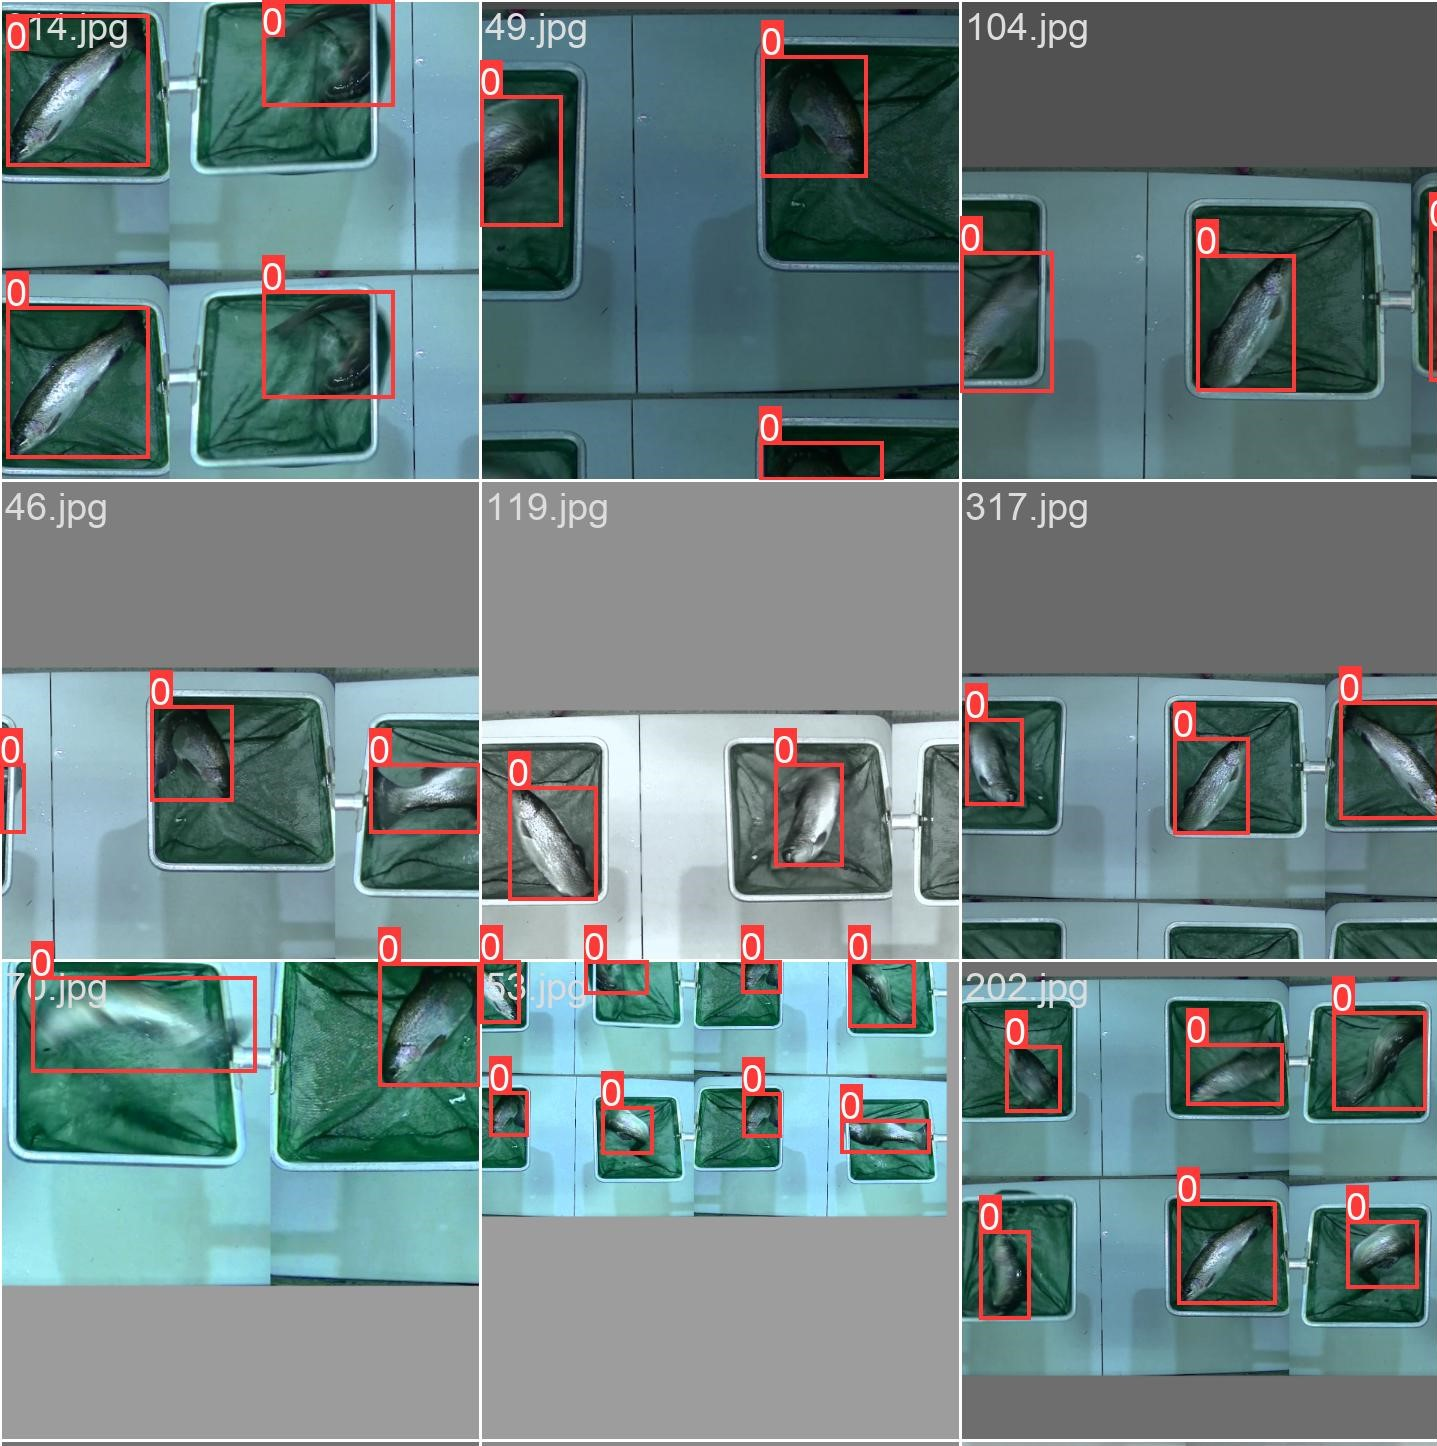
\includegraphics[width=0.7\textwidth]{images/13/a/EjemploAumento.jpg}
    \caption{Ejemplo de aumento de datos automático de \texttt{YOLO}}
    \label{fig:AumentoDatosYolo}
\end{figure}
\clearpage
Aparte de los posibles ajustes de hiperparámetros, es necesario explicar los estadísticos que se obtienen de realizar un entrenamiento con un modelo \texttt{YOLO}. En el caso de este trabajo, se realizará una 
explicación de los resultados que devuelve un modelo de detección.

Las métricas que se tienen en cuenta durante el entrenamiento son:

\begin{itemize}
    \item \textbf{Box Loss sobre el conjunto de entrenamiento}: representa el error del tamaño y posición de las \texttt{Bounding Boxes} de las etiquetas sobre las predichas en cada época. Cuando menor sea, 
    mayor es la cercanía entre las cajas predecidas en el conjunto de entrenamiento respecto a sus etiquetas reales.\newline Una representación de un cálculo simple de este valor se puede ver en la \autoref{fig:IoU}, a través de la 
    intersección entre unidad, cuanto más cerca esté de 1, mejor.

    \begin{figure}[H]
        \centering
        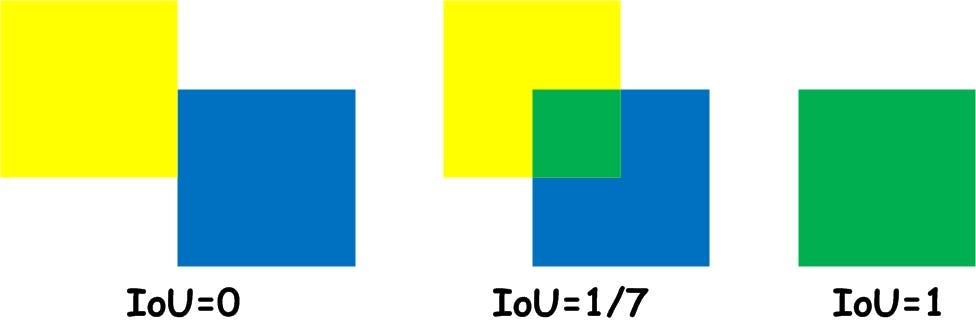
\includegraphics[width=0.5\textwidth]{images/13/a/IoU.png}
        \caption{Factor IoU para calcular la perdida de cajas en una \texttt{CNN} de detección}
        \label{fig:IoU}
    \end{figure}
    \item \textbf{Cls Loss sobre el conjunto de entrenamiento}: representa el error de clasificación de cada objeto detectado en la imagen respecto al de la etiqueta real en el conjunto de entrenamiento.
    \item \textbf{Dfl Loss sobre el conjunto de entrenamiento}: es un error sobre la capacidad del modelo \texttt{YOLO} para soportar deformaciones de los objetos detectados.
    \item \textbf{Precisión (B)}: indica la precisión general sobre los objetos detectados, para realizar este cálculo se tienen en cuenta todas las métricas anteriores como una media con pesos y condiciones. Idealmente es 1 como máximo.
    \item \textbf{Recall (B)}: indica la capacidad que se ha tenido para detectar todas las instancias, se utiliza despues para saber cuantos elementos detecta con una precisión determinada. Idealmente es 1.
    \item \textbf{Métrica \acrshort{map}50 (B)}
    \item \textbf{Métrica \acrshort{map}50-95 (B)}
    \item \textbf{Box Loss sobre el conjunto de validación}
    \item \textbf{Cls Loss sobre el conjunto de validación}
    \item \textbf{Dfl Loss sobre el conjunto de validación}
\end{itemize}

\clearpage
\subsection*{ANEXO B: Datos de entrenamiento}
\label{subsec:B}